\chapter{\ifenglish Background Knowledge and Theory\else ทฤษฎีที่เกี่ยวข้อง\fi}

% การทำโครงงาน เริ่มต้นด้วยการศึกษาค้นคว้า ทฤษฎีที่เกี่ยวข้อง หรือ งานวิจัย/โครงงาน ที่เคยมีผู้นำเสนอไว้แล้ว ซึ่งเนื้อหาในบทนี้ก็จะเกี่ยวกับการอธิบายถึงสิ่งที่เกี่ยวข้องกับโครงงาน เพื่อให้ผู้อ่านเข้าใจเนื้อหาในบทถัดๆ ไปได้ง่ายขึ้น
\par โครงงานนี้ได้นำองค์ความรู้ในด้านของ Computational Intelligence และ การ streaming แบบ Peer-to-peer   
ของรูปภาพจาก application ไปยัง backend ผ่าน WebRTC (Web Real Time Communications) เพื่อให้ backend 
ที่เป็น Computational Intelligence ทำการ classification products  
  
  
\section{WebRTC for Streaming image}
\par WebRTC (Web Real-Time Communication) เป็น open-source  ที่ให้บริการ  web browsers
 และ mobile applications ด้วยการสื่อสารแบบเรียลไทม์ (RTC) ผ่าน (API)  
 ทำให้การ Communication ด้วยเสียงและวิดีโอได้ผ่าน  Peer-to-peer   โดยตรงตามรูป \ref{fig:webrtc structure}
 
 
\begin{figure}[h]
\begin{center}
% 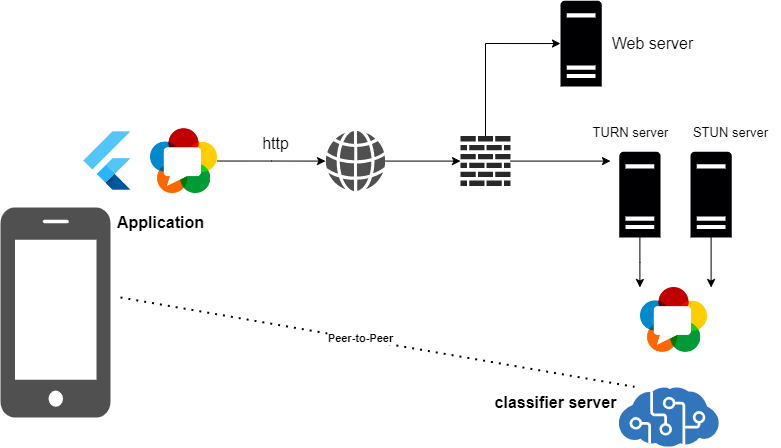
\includegraphics{pic/webrtc.png}
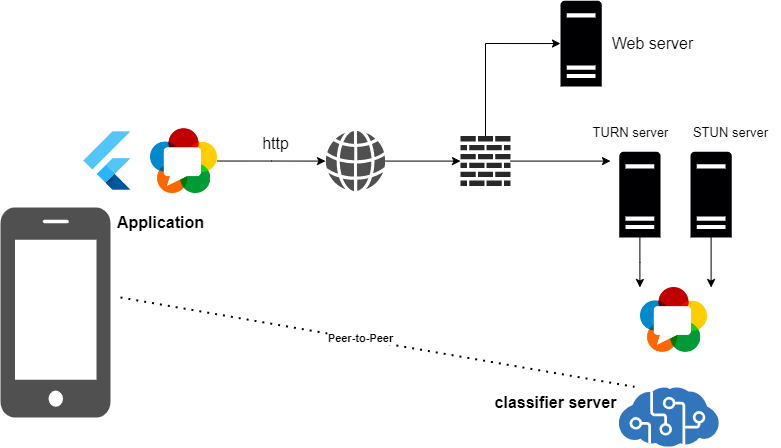
\includegraphics[scale=0.5]{pic/webrtc.png}
\end{center}

\caption[webrtc structure]{webrtc structure}
\label{fig:webrtc structure}
\end{figure}



\section{Artificial neural networks} 
% Deep Learning is the branch of Machine Learning based on Deep Neural Networks (DNNs), 
% meaning neural networks with at the very least 3 or 4 layers (including the input and output layers). 
\par เป็นแขนงหนึ่งของ Computational Intelligence ซึ่งได้รับแรงบรรดาลใจมาจากการทำงานของสมองของมนุษย์
ซึ่งประกอบด้วยหน่วยเล็กๆ เรียกว่า cell Neuron แต่ละ Neuron ก็จะเชื่อมต่อโยงใยกันด้วยเส้นประสาทเรียกว่า ไซแนปส์ (Synapse) เพื่อส่งสัญญาณไฟฟ้า ที่เกิดจากสิ่งเร้าต่างๆ ว่าจะตอบสนองต่อสิ่งเร้านั้นอย่างไร 
โดยแต่ละ Neuron จะได้รับ Input หลาย ๆ อัน จากกิ่งก้านสาขาของ Dendrite แล้วนำมาประมวลผล ออกมาเป็น 1 Output ออกไปที่ Axon เพื่อส่งต่อไปให้ Dendrite ของ Neuron อื่น ๆ ใช้เป็น Input ต่อไป

เมื่อมนุษย์เติบโดขึ้น หาก Neuron ไหนตอบสนองต่อสิ่งเร้าประเภทไหนได้ดี ก็จะสามารถส่งสัญญาณไฟฟ้าได้แรง มากกว่า Neuron อื่นๆ
เมื่อ Neuron หลายๆอันต่อกันหลายๆ layer ก็จะกลายเป็น Neuron network ของมนุษย์

โดยในทาง  Computational Intelligence จะใช้ node เป็นตัวแทนของ Neuron โดยจะเรียงเป็นชั้นๆ (layer) 
โดยสัญญาณที่ส่งออกจากแต่ละ node จะมี weight ที่กำหนดความแรงของสัญญาณนั้นๆ เมื่อมีหลายๆ node และต่อกันหลายๆ layers
ก็จะกลายเป็น neural network ขนาดใหญ่ เรียกว่า deep learning ซึ่งเลียนแบบการการทำงานของสมองมนุษย์
ทำให้  computers สามารถ process ข้อมูลในลักษณะเดียวกับที่ สมองของมนุษย์ทำการประมวณผลข้อมูล 

\subsection{Multilayer perceptron}
เป็นส่วนพื้นฐานของ neural network เป็นการ ที่ node ในแต่ละ layer เชื่อมต่อกับ ทุก node ของ layer+1 (fully connected)
โดยทุกเส้นการเชื่อมต่อของ $node_i$  กับ $node_j$ จะมี weight $w_{ji}$  ซึ่งเป็นความแรงของสัญญาณอยู่ 
\\ โดยจะมี Input layer สำหรับรับข้อมูล (สิ่งเร้า) , hidden layer ในการตัดสินใจ , output layer ในการเลือกการกระทำกับสิ่งเร้านั้นๆ
\begin{figure}[h]
  \begin{center}
  % 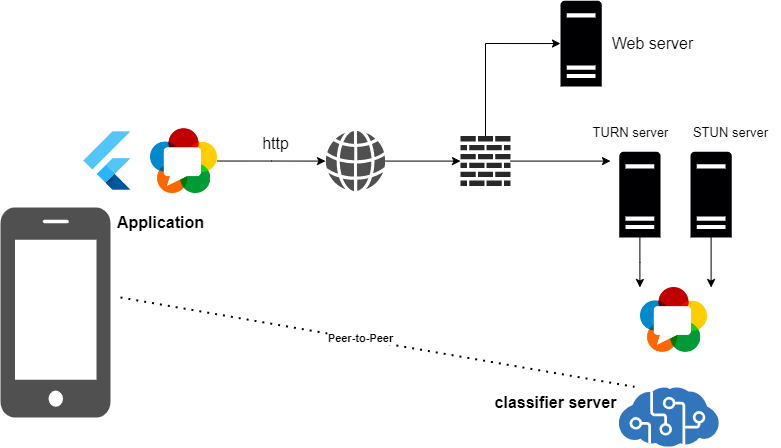
\includegraphics{pic/webrtc.png}
  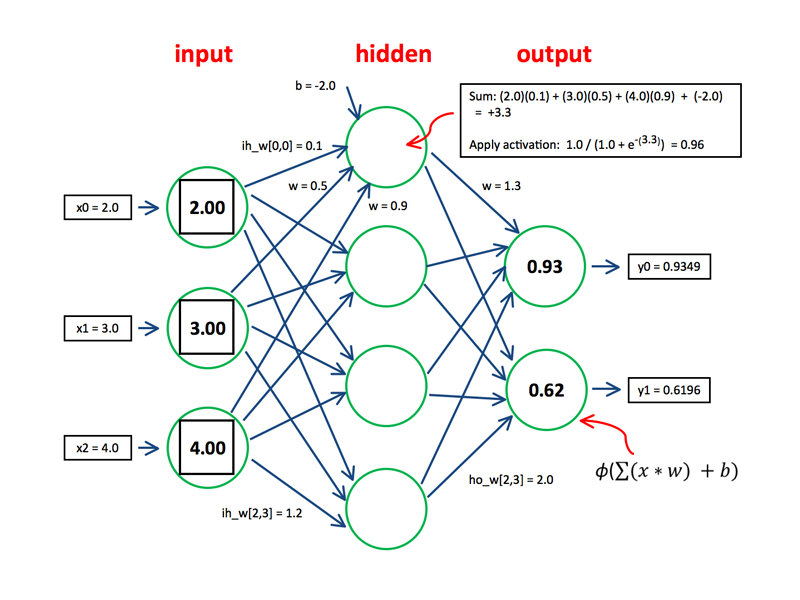
\includegraphics[scale=0.5]{pic/mlp.png}
  \end{center}
  % https://visualstudiomagazine.com/articles/2013/05/01/neural-network-feed-forward.aspx
  \caption[Multilayer perceptron]{Multilayer perceptron}
  \label{fig:Multilayer perceptron}
  \end{figure}

โดยในแต่ละ node ที่ไม่ใช่ Input layer จะรับค่าผลรวมจาก node ก่อนหน้า เป็นผลรวมจากทุก Input (ทุก Dendrite) ของ node นั้นๆ
\newline
โดยสมการ Input \begin{equation} node_j  =  v_j = \sum(\forall w_{j_i})+biase \end{equation}

Activation function คือ ฟังก์ชันที่รับ ผลรวมจากทุก Input ( $v_j $)  แล้วคำนวณว่าจะส่งต่อเป็น Output เท่าไร
ซึ่งมี function มากมายไม่ว่าจะเป็น Hyperbolic tangent ,Sigmoid , ReLU

โดยในทุกๆ $node_j$ จะมี Activation function สำหรับคำนวณค่า output ที่จะส่งต่อไปยัง layer ถัดไป  
% \textrm{and}

\begin{equation} output node_j =  Y_j =  y(v_i)  \end{equation}
 โดยที่  \begin{equation} ~~ y(v_i) = \begin{cases}
  \tanh(v_i)  & \text{,Hyperbolic Activation function} \\
  (1+e^{-v_i})^{-1} & \text{,Sigmoid Activation function} \\
  \max(0,v_i) & \text{,Sigmoid Activation function}\\
  \text{etc } & \text{, etc }\\
  \end{cases} \end{equation}
%  \newline โดยที่  $ ~~ y(v_i) = \tanh(v_i)   $      สำหรับ  Hyperbolic tangent Activation function
%  \newline โดยที่   $ ~~ y(v_i) = (1+e^{-v_i})^{-1}$ สำหรับ  Sigmoid Activation function
%  \newline โดยที่   $ ~~ y(v_i) = \max(0,v_i)$       สำหรับ  ReLU Activation function

% เป็นการเรียนรู
% คือวิธีการเรียนรู้แบบอัตโนมัติด้วยการ เลียนแบบการทำงานของโครงข่ายประสาทของมนุษย์ (Neurons) โดยนำระบบโครงข่ายประสาท (Neural Network) มาซ้อนกัน หลายชั้น (Layer) และทำการเรียนรู้ข้อมูลตัวอย่าง ซึ่งข้อมูล ดังกล่าวจะถูกนำไปใช้ในการตรวจจับรูปแบบ (Pattern) หรือจัด หมวดหมู่ข้อมูล (Classify the Data)
\subsection{Classification}
จาก Input layer ข้อมูลจะถูกส่งต่อไปยัง layer ถัดๆไป เรียกว่า Passed forward และเมื่อถึง
layer สุดท้ายของ neural network เรียกว่า output layer โดยส่วนใหญ่ใน output layer นี้จะมีจำนวนของ node เท่ากับจำนวนของ class ของข้อมูลที่จะทำการ classification 
โดยแต่ละ node ใน output layer จะเป็นตัวแทนของ class ซึ่ง หาก node ใดให้ค่า output node เยอะที่สุด input data ก็ถูก classify เป็น class ของ node นั้นๆ


\subsection{Training}
คือการ train โดยใช้ dataset เปลี่ยน weight ในแต่ละเส้นของ MLP เพื่อให้ตอบสนองต่อ Input ให้ใกล้เครียงกับสิ่งที่ควรจะเป็นมากขึ้น 
โดยหนึ่งในวิธีการเปลี่ยน weight คือ backpropagation
 

โดยค่า error ที่ได้มาจาก output layer กับ ค่าที่ควรได้จาก Input ที่ใส่เข้าไป เพื่อเปลี่ยน weight ให้ค่า error มีค่าน้อยลงกว่าเดิม
\begin{equation} output node_j =  Y_j =  y(v_i)  \end{equation}

 สามารถคำนวณหาค่า error ในแต่ละ node ของ output layer ได้โดย
 \begin{equation}  e_j(n)=d_j(n)-y_j(n) 
 \end{equation}
 where $d_{j}(n)$  is the desired target value , and $y_{j}(n)$   value produced by the perceptron at $node_j$


%  หรือทำให้ output node ใน layer output ที่เป็น class ของ input นั้นๆ มีค่าเยอะที่สุด
 
\begin{equation} 
{\displaystyle {\mathcal {E}}(n)={\frac {1}{2}}\sum _{{\text{output node }}j}e_{j}^{2}(n)}.
\end{equation} 
และใช้  gradient descent ในการเปลี่ยน weight ในแต่ละเส้น
\begin{equation} 
\Delta w_{ji} (n) = -\eta\frac{\partial\mathcal{E}(n)}{\partial v_j(n)} y_i(n)
\end{equation} 


\newpage


เนื่องจาก train dataset นั้นมีขนาดที่ใหญ่เกินไป จึงมีการแบ่ง dataset ให้เล็กลง ซึ่งจะมีคำศัพท์ ดังนี้

\begin{enumerate}
  \item Epoch :  โดยจาก train dataset  1 Epoch คือการที่ dataset ทั้งหมด Passed forward และ backpropagation
  \item Batch Size : แบ่ง dataset เป็น set ขนาดๆ ย่อยๆ 
  \item Iterations : จำนวน Batch ที่ต้องใช้เพื่อที่จะครบ 1 Epoch
\end{enumerate} 
 
 
\section{Convolutional neural network}
เป็น Computational intelligence ที่ออกแบบมาในงานด้านรูปภาพ 
ใช้การดำเนินการที่เรียกว่า "convolution"  (สัญลักษณ์ *) เป็นการดำเนินการทางคณิตศาสตร์ ระหว่างสองฟังก์ชัน f * g เพื่อดูการเปลี่ยนแปลงของฟังก์ชัน (f) เมื่อมีฟังก์ชัน (g) เข้ามา 
ใช้ในการเพื่อประมวลผลข้อมูลภาพ  
\begin{equation}
   {\displaystyle (f*g)(t):=\int _{-\infty }^{\infty }f(\tau )g(t-\tau )\,d\tau .}
\end{equation} 
 
โดยจะแบ่งส่วนของภาพเป็นส่วนย่อยๆ ไปทั่วทั้งรูปภาพ แล้วนำไป convolution กับ  "filters" หรือที่เรียกว่า "kernels" เพื่อหา patterns ของรูปภาพ ที่เรียกว่า feature map
\begin{figure}[h]
  \begin{center}
  % 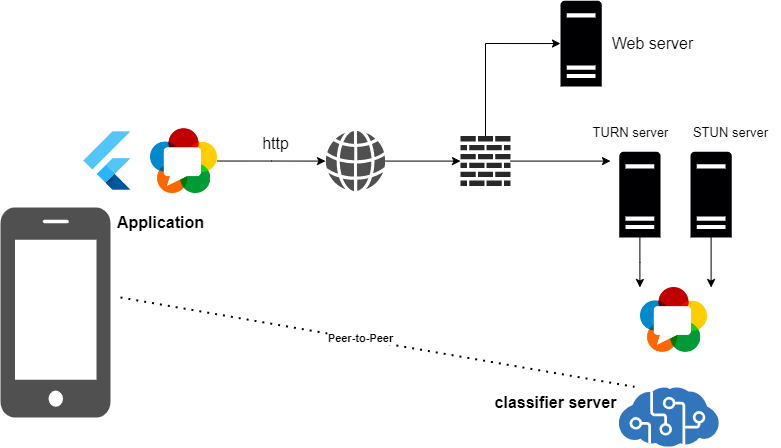
\includegraphics{pic/webrtc.png}
  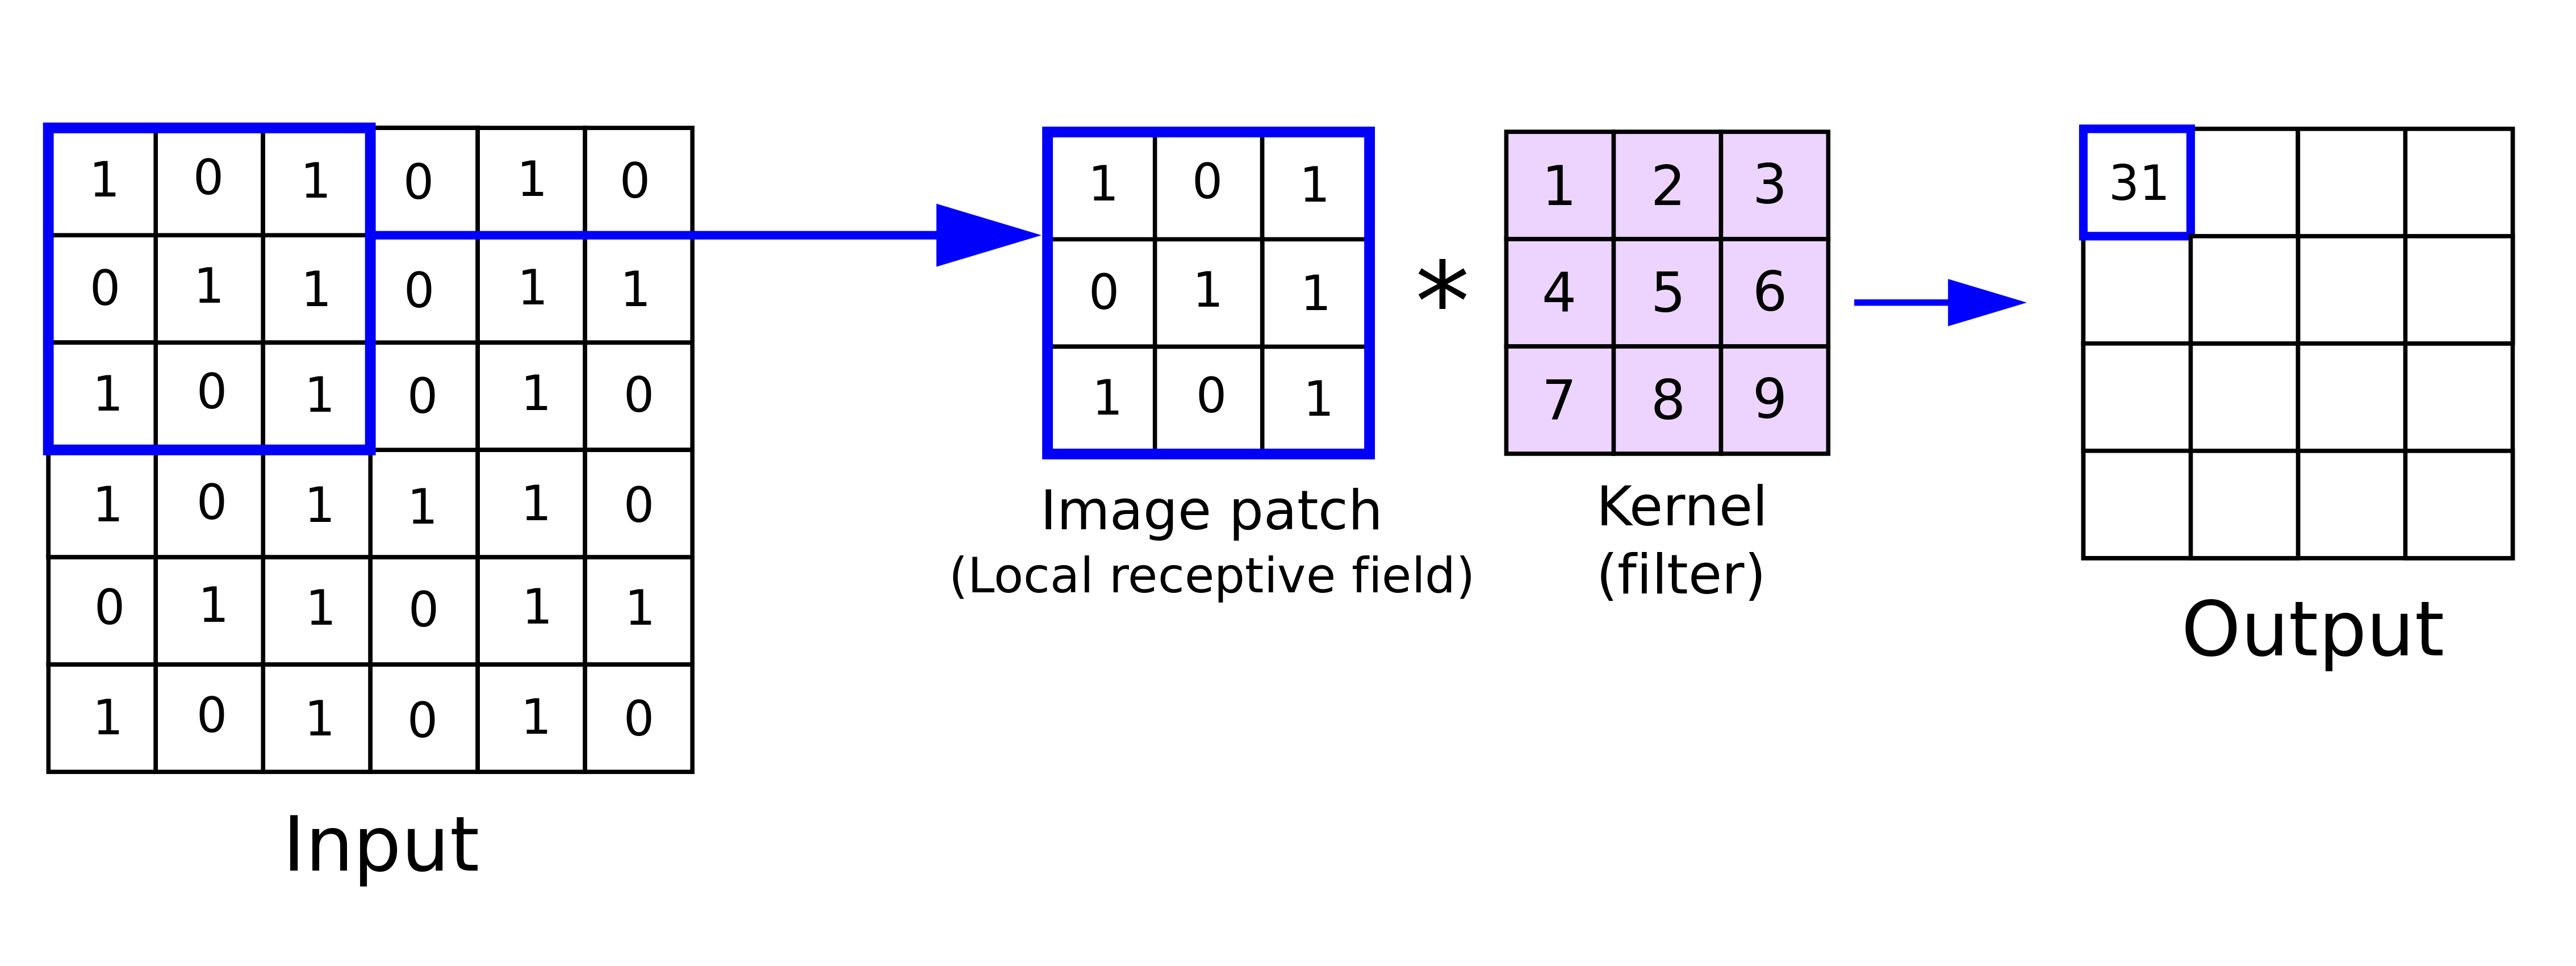
\includegraphics[scale=0.05]{pic/cnn.png}
  \end{center}
  %  https://anhreynolds.com/blogs/cnn.html
  \caption[Convolution]{Convolution}
  \label{fig:Convolution }
  \end{figure}


CNNs ต่างจาก neural networks อื่นๆ ตรงที่  shared-weight ร่วมกัน ซึ่งทำให้มีความสามารถในการแยกแยะ patterns ได้ดี


หากเขียนในรูปแบบ Neural network
\begin{figure}[h]
  \begin{center}
  % 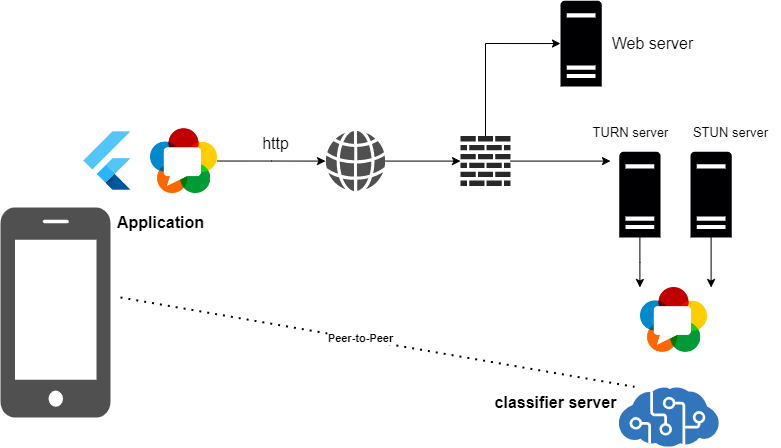
\includegraphics{pic/webrtc.png}
  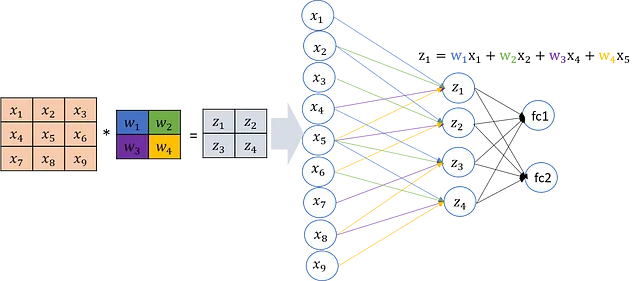
\includegraphics[scale=0.45]{pic/cnn_nn.png}
  \end{center}
% https://medium.com/@hadee2531earvesdrop/convolutional-neural-network-%E0%B8%84%E0%B8%B7%E0%B8%AD%E0%B8%AD%E0%B8%B0%E0%B9%84%E0%B8%A3-42c45f7ec16b

  \caption[Convolutional neural network]{Convolutional neural network }
  \label{fig:Convolutional neural network }
  \end{figure}


\section{Transfer learning}


% \section{Transfer Learning}
 
% Section 2 text.

% \section{Transfer Learning}
เป็นเทคนิคที่นำ model ที่ผ่านการฝึกฝนจนแก้ ปัญหาในงานอื่นๆที่มีความคล้ายคลึงกัน
นำมาเป็น model ตั้งต้น สำหรับ model ในการแก้ปัญหาใหม่ๆ
ตัวอย่างเช่น โมเดลที่ได้รับการฝึกฝนให้จดจำวัตถุในภาพสามารถใช้
เพื่อระบุวัตถุที่คล้ายกันในภาพต่างๆ ได้ 
แม้ว่าภาพใหม่จะมีสภาพแสงหรือพื้นหลังต่างกันก็ตาม
 กุญแจสำคัญคือการระบุคุณสมบัติทั่วไปหรือการเป็นตัวแทนที่ใช้ร่วมกันระหว่างโดเมนต้นทางและโดเมนเป้าหมาย
 วิธี Transfer Learning ที่ได้รับความนิยมมากที่สุดวิธีหนึ่งคือ fine-tuning 
คือการใช้โมเดลที่ผ่านการ  pre-trained  มาแล้ว นำมา train ต่อบน ชุดข้อมูลใหม่
และใช้ learning rate น้อยๆ เพื่อป้องกัน weight ที่เคยผ่านการ train จนมีความแม่นยำเปลี่ยนแปลงไปมาก จนไม่มีความแม่นยำ
อีกวิธีหนึ่งคือ feature extraction ซึ่งเกี่ยวข้องกับการใช้ โมเดลที่ผ่านการ  pre-trained  เป็นตัวแยกคุณลักษณะของ ข้อมูล และ สร้าง model ใหม่เพื่อ train จากคุณลักษณะเหล่านี้ที่ model ตั้งต้นแบ่งแยกออกมาได้
 
% \subsection{Transfer Learning}
\begin{figure}[h]
  \begin{center}
  % 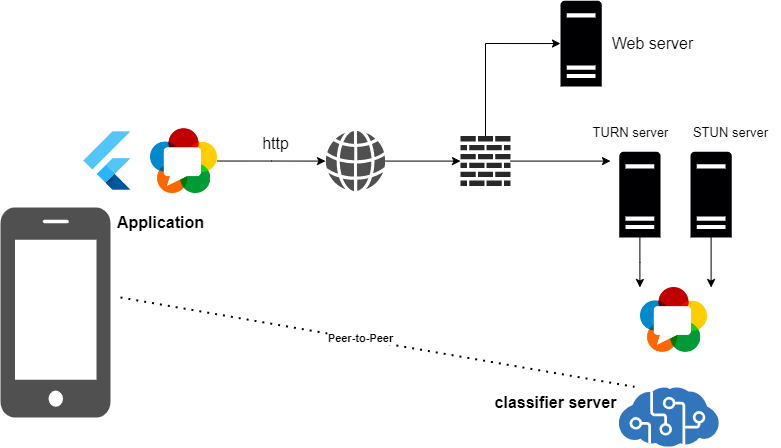
\includegraphics{pic/webrtc.png}
  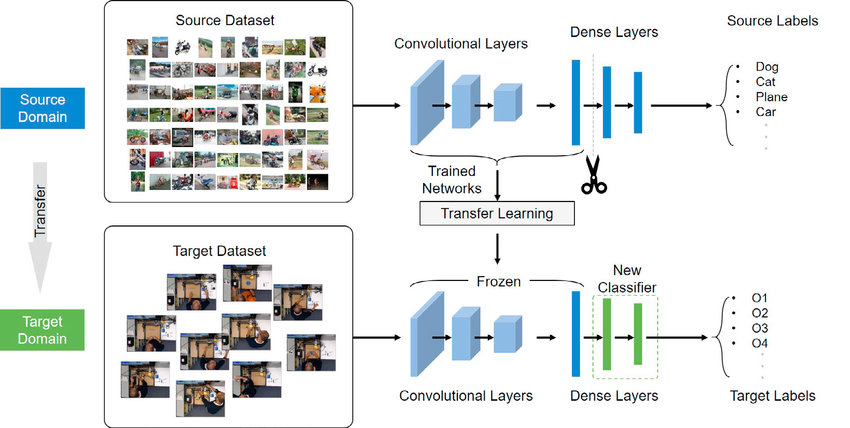
\includegraphics[scale=0.45]{pic/The-architecture-transfer-learning.png}
  \end{center}
  
  \caption[The concept of transfer learning]{The concept of transfer learning}
  \label{fig:The concept of transfer learning}
  \end{figure}

  \subsection{transfer learning - Xception}
  โดย model pre-train 'Xception' เป็น convolutional neural network ซึ่งมมีความลึก 71 layers.
เป็นโมเดลที่ผ่านการจากรูปภาพต่างๆ มากกว่าล้านรูปภาพจาก ImageNet database [1].


  ซึ่งสามารถ
\begin{center}
  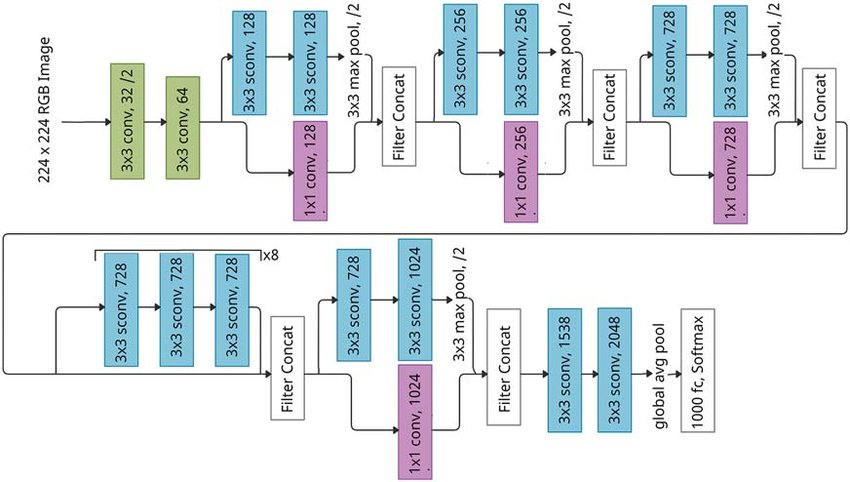
\includegraphics[scale=0.35]{pic/x.png}
\end{center}
% \section{classification products}

% \section{web dashboard}
% Section 3 text. The dielectric constant\index{dielectric constant}
% at the air-metal interface determines
% the resonance shift\index{resonance shift} as absorption or capture occurs
% is shown in Equation~\eqref{eq:dielectric}:

% \begin{equation}\label{eq:dielectric}
% k_1=\frac{\omega}{c({1/\varepsilon_m + 1/\varepsilon_i})^{1/2}}=k_2=\frac{\omega
% \sin(\theta)\varepsilon_\mathit{air}^{1/2}}{c}
% \end{equation}

% \noindent
% where $\omega$ is the frequency of the plasmon, $c$ is the speed of
% light, $\varepsilon_m$ is the dielectric constant of the metal,
% $\varepsilon_i$ is the dielectric constant of neighboring insulator,
% and $\varepsilon_\mathit{air}$ is the dielectric constant of air.

% \section{About using figures in your report}

% define a command that produces some filler text, the lorem ipsum.
% \newcommand{\loremipsum}{
%   \textit{Lorem ipsum dolor sit amet, consectetur adipisicing elit, sed do
%   eiusmod tempor incididunt ut labore et dolore magna aliqua. Ut enim ad
%   minim veniam, quis nostrud exercitation ullamco laboris nisi ut
%   aliquip ex ea commodo consequat. Duis aute irure dolor in
%   reprehenderit in voluptate velit esse cillum dolore eu fugiat nulla
%   pariatur. Excepteur sint occaecat cupidatat non proident, sunt in
%   culpa qui officia deserunt mollit anim id est laborum.}\par}

% \begin{figure}
  % \centering

  % \fbox{
    %  \parbox{.6\textwidth}{\loremipsum}
  % }

  % To include an image in the figure, say myimage.pdf, you could use
  % the following code. Look up the documentation for the package
  % graphicx for more information.
  % \includegraphics[width=\textwidth]{myimage}

  % \caption[Sample figure]{This figure is a sample containing \gls{lorem ipsum},
  % showing you how you can include figures and glossary in your report.
  % You can specify a shorter caption that will appear in the List of Figures.}
  % \label{fig:sample-figure}
% \end{figure}

% Using \verb.\label. and \verb.\ref. commands allows us to refer to
% figures easily. If we can refer to Figures
% \ref{fig:walrus} and \ref{fig:sample-figure} and \ref{fig:webrtc}  by name in the {\LaTeX}
% source code, then we will not need to update the code that refers to it
% even if the placement or ordering of the figures changes.

% \loremipsum\loremipsum

% This code demonstrates how to get a landscape table or figure. It
% uses the package lscape to turn everything but the page number into
% landscape orientation. Everything should be included within an
% \afterpage{ .... } to avoid causing a page break too early.
% \afterpage{
%   \begin{landscape}
%   \begin{table}
%     \caption{Sample landscape table}
%     \label{tab:sample-table}

%     \centering

%     \begin{tabular}{c||c|c}
%         Year & A & B \\
%         \hline\hline
%         1989 & 12 & 23 \\
%         1990 & 4 & 9 \\
%         1991 & 3 & 6 \\
%     \end{tabular}
%   \end{table}
%   \end{landscape}
% }

% \loremipsum\loremipsum\loremipsum

% \section{Overfull hbox}

% When the \verb.semifinal. option is passed to the \verb.cpecmu. document class,
% any line that is longer than the line width, i.e., an overfull hbox, will be
% highlighted with a black solid rule:
% \begin{center}
% \begin{minipage}{2em}
% juxtaposition
% \end{minipage}
% \end{center}

% \section{\ifenglish%
% \ifcpe CPE \else ISNE \fi knowledge used, applied, or integrated in this project
% \else%
% ความรู้ตามหลักสูตรซึ่งถูกนำมาใช้หรือบูรณาการในโครงงาน
% \fi
% }

% อธิบายถึงความรู้ และแนวทางการนำความรู้ต่างๆ ที่ได้เรียนตามหลักสูตร ซึ่งถูกนำมาใช้ในโครงงาน

% \section{\ifenglish%
% Extracurricular knowledge used, applied, or integrated in this project
% \else%
% ความรู้นอกหลักสูตรซึ่งถูกนำมาใช้หรือบูรณาการในโครงงาน
% \fi
% }

% อธิบายถึงความรู้ต่างๆ ที่เรียนรู้ด้วยตนเอง และแนวทางการนำความรู้เหล่านั้นมาใช้ในโครงงาน
